\chapter{Methodological approach}
- (3h) Writing Process: Go through markdown notes (prepare writing)
- (2h+) Refactoring: Start Camunda Modeler (see whether it works)
	-> Look at results for next steps


\section{Motivation and Procedure}
% 
% What we did so far: Transition
% 

%
% Goals and Priority
%


% Primary Goal is to do the Refactoring Process

% TODO: Formulate this caveat after writing the business case
	% Business Case will not be covered, technical debt will not be estimated.
	% - But: Software Project will be transformed in future
	% - Thus: By the detection of internal problems coupled future development,
	% 	refactoring seems to be self-evident.

% Note: Reworking the entire Application is not in the scope of the thesis

% Secondary Goals - Discussion part
Whereas primary ...





% ------------------------------------------------------------------------
% Hypotheses
% ------------------------------------------------------------------------
Based on these goals -> constucted following hypotheses.

During the practical work, 
	the thesis will try to validate two types of hypotheses.


% ------------------------------------------------------------------------
% Transition: Short Overview of Procedure
% ------------------------------------------------------------------------

\section{Analysis: Detecting Code Smells}

% Introduction Paragraph
The following part of this chapter moves on to describe in greater detail detection code smells within the software system. It provides a brief overview of the methods used for detection and mentions the prevalence of sonargraph as the main suite of software products utilized in the detection activities. Moreover, this section provides some clarifications necessary to comprehend certain methods to be chosen over others.

% Catalogue
Out of 24 code smells that are examined throughout Martin Fowler's book on refactoring, only 10 are chosen to be included in the detection work. Further, the 2 smells \emph{refused bequest} and \emph{data clumps} were discarded, as their focus on inheritance and data structures respectively, are not utilized in the code. In order to revisit the code smell catalog with their corresponding explanation, refer to (sec:...)
 

% Restrictions
There exists several reasons that have led to the decision of restricting the amount of smells for this section. First, it is not the scope of the thesis to find every code smell in the codebase. Finding and evaluating each smell that is known in literature would be a tedious task, as there are no automatic tools available for the python programming language, as will be discussed in a later part of this section. Hence, it suffices, if some smells that are prevalent have been detected. In addition, it is also advantageous to only focus on the most prominent smells. Very niche smells could distract from improving the quality of the entire code base, as well as provide less of possibilities to make generalizations.

% Metrics based
Many tools have been created to automatically or semi-automatically detect code smells (Menshawy, p.1). In the context of our paper, the code smells are detected semi-automatically using a metric-based approach. This approach measures source code elements and takes decisions based on threshold values (Menshawy, p.4) It is fulfills two requirements necessary for the following work. On the one hand, it to a certain degree contains automation, making it much more efficient in comparison to manual approaches. On the contrary, it can be used for the python programming language, which is essential in the software system at hand. Menshawy points out (p.3) that with metrics approach does not provide metrics for every code smells. Nevertheless, for the eight smells the thesis is focussing on, as will be seen afterwards, an appropriate metric was found.

% Automation based
Using a detection approach based on automated tools would have been more attractive, but unfortunately not possible.  It is the most used approach (Menshawy, p.2), its availability is however highly dependent on the programming language the software system is written in (Menshawy, p.3). By looking at Menshawy's research (p.3) on most cited tools, it can be observed that a significant difference exists between java programming language, which was supported  by 48\% of the tools, whereas the python programming language being only supported by 4\%.
In addition, by researching automated tools appropriate for python, it was evident that at this moment of time, the offering is insufficient for to accomplish a sound detection strategy. 

% Manual approach
In the beginning, the author has also considered following a manual approach. In contrast to automation, the manual detection relies on human perception of smells by applying predefined guidelines (Menshawy, p.3). It is characterized as highly time-consuming and prone to human error. Therefore, when comparing this approach to a metrics-based, it is a less desirable way for detecting smells and was subsequently discarded as a detection technique.

% Visualization
Another detection approach that has not yet been mentioned, is using visualization. Although it only is used to detect a subset of smells, visualization had been used in two occurrences throughout the thesis. First, it had been used to get a broad overview of the code base, which helped the author as an orientation. Second, it was used [... Add coupling + cohesion]

% Intro Sonargraph
The detection of code smells relied heavily on a code analyzer tool called sonargraph. It demonstated to be extremely useful in the detection of code smells, by its ability to compute and list metrics of the software system. Countless metrics offered a diversity of selection, analyzing both on the basis of the entire project and individual modules. By reading through the the provided explanations of the metric an appropriate metric could be found for all of the desired code smells relevant for the thesis.

% Explorer + Metrics
Compared to other software solutions, sonargraph was chosen for several reasons. Altough its entire product suite is not, its graphical application "Explorer" was free to use. For the thesis it provided many ways to make observations about the code base, including numerical and visual methods. All the tools needed to compute metrics were restricted in this free application of the product family. In contrast, the detection of code duplication was not included within "Explorer". Nevertheless, altough unsure about the amount, it was possible to renew a trial period multiple times. Hence, in order to recreate this method one must be aware of this restriction. Another noteworthy benefit of using sonargraph during the detection, was its ability to observe the entire project,  and not just at individual files. This was essential for metrics taking account of dependencies between modules. In addition, it was beneficial not to rely on a multitude of software tools, by having just one software.



\begin{figure}[htp]
    \centering
    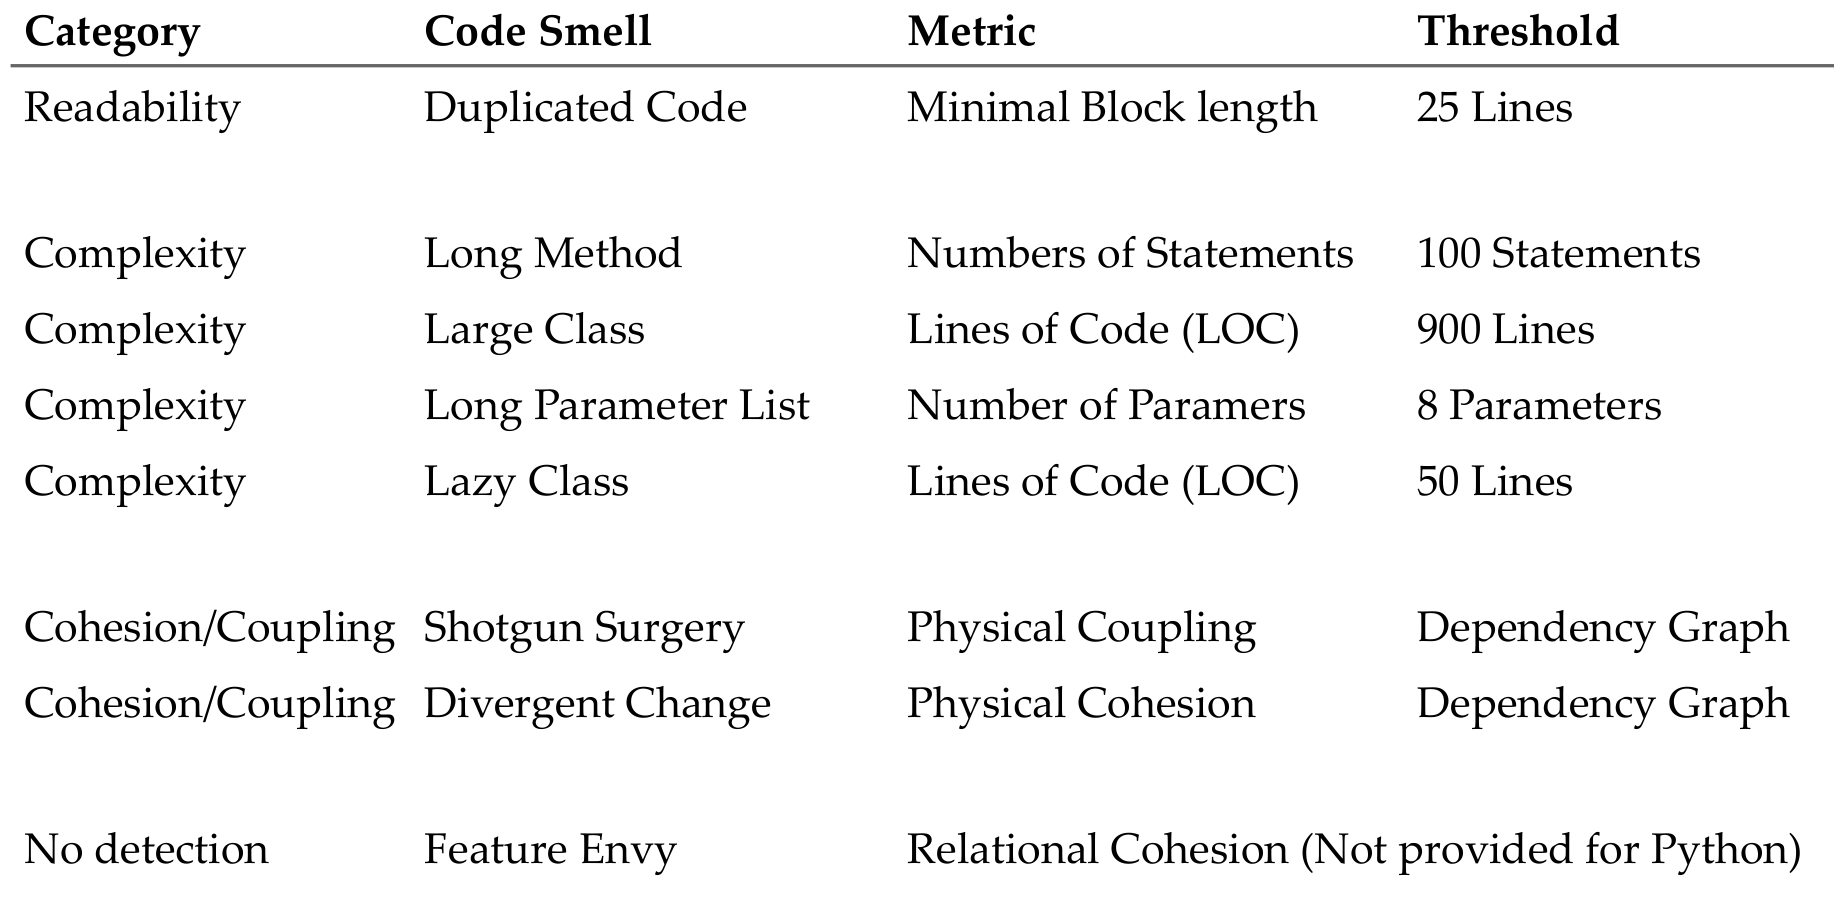
\includegraphics[width=\textwidth]{./assets/smell_overview}
    \caption{Metrics without prioritization}
\end{figure}
% Table
The above table presents for each code smell a corresponding metric. In addition, for some metrics, a threshold value is given. When the threshold value is surpassed, there is an indication that this code smell exists in the software system.

% Subgroups
Individual metrics are categorized into three subgroups, named after the quality attribute they best represent. More importantly, however, this distinction is made, as each of the group differs in regard to how a metric results in a smell detected. 

% Duplicated Code -> Automated
Duplicate code particularly differs from the other smells, due to it being detected automatically. Previously, it was stated that it was difficult to find appropriate tools to detect code smells, due to lack of availability.
In the case of code duplication, this is however readily available because detecting code duplication can be done language agnostic. In order to detect duplication of code in programs, the software does not need to understand the programming language. For instance, this same mechanism could be applied to other types of text that are not code.

% Complexity -> Threshold
Half of the code smells, in the subgroup called complexity, follow a typical metrics based approach. The threshold value indicate when a code smell is potentially present. Notably, all the metrics in this category involve counting of some sorts. In particular, the smells are detected by counting the number of statements, lines of codes, and numbers of parameters of methods. Prioritization of given smells can be done by comparing the extent of how much a given threshold value is surpassed. Similarly, code smells can be discarded if the associated metric does not surpass the threshold value. 

% Cohesion/Coupling -> Dependency graph
[Don't know yet]
- For Shotgun Surgery and Divergent change, a dependency graph will be used in addition to the metric.
- Sonargraph does not provide a threshold value.
	-> This allows to evaluate the amount of dependencies in relation to the entire project in order to see any outlying behavior


\section{Testing: Framework}

\section{Measurment: Success}

\section{Implementation: Refactor}

\section{Extra Activities}

\section{Limitations and justification}
